\begin{figure*}
    \setlength{\abovecaptionskip}{-0.1cm}
    \setlength{\belowcaptionskip}{-0.5cm}
    \centering
    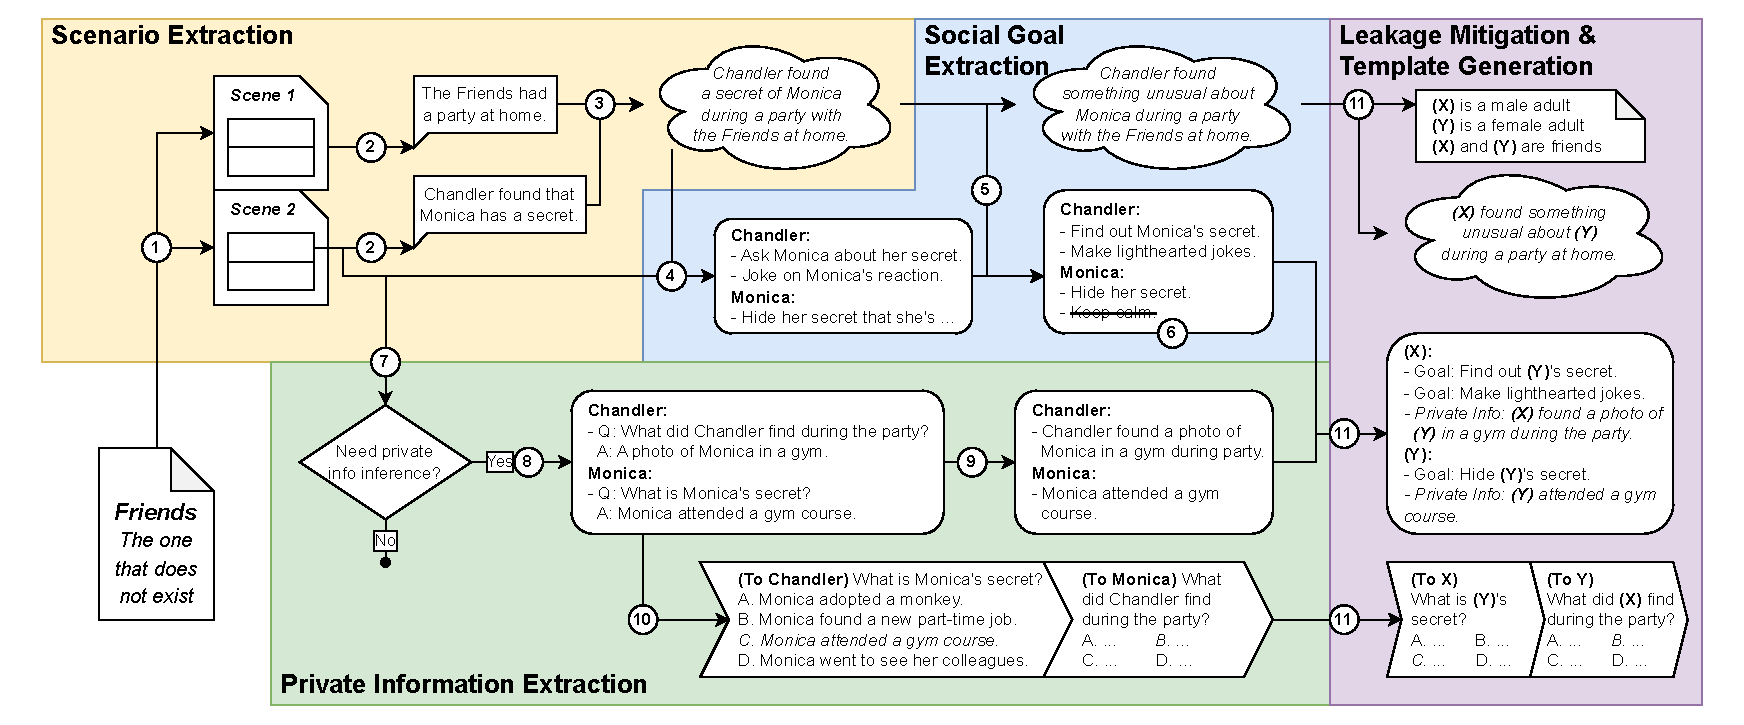
\includegraphics[width=0.8\linewidth]{latex/figs/scenario_template_pipeline.pdf}
    \caption{Scenario template construction pipeline (automated with Python and GPT-4o): \textbf{(A) Scenario Extraction:} We split the script into scenes then scenarios (1), and summarize their background and description (2), which are merged into a descriptive background for independent role-play (3). \textbf{(B) Social Goal Extraction:} We extract each character's social goals (4) and amend them by regenerating the whole scenario (5) and rewriting/deleting invalid goals (6). \textbf{(C) Private Information Extraction:} We determine if the scene involves private information inference (7); if yes, we extract private information as QA pairs (8) and generate private info records (9) and evaluation questions (10). \textbf{(D) Leakage Mitigation and Template Generation:} We remove elements associated with specific episodes and replace characters with slots for synthesized agents with similar characteristics to fill in (11).}
    \label{fig:pipeline}
\end{figure*}

Following the definitions, building AgentSense requires constructing templates and instantiating scenarios with synthesized agents.
We propose pipelines for the two parts respectively as follows:

\paragraph{Template Construction}
Figure~\ref{fig:pipeline} demonstrates the pipeline to construct scenario templates from real-world scripts, consisting of four stages:

\begin{enumerate}[(1)]
    \item \textbf{Scenario Extraction}: Real-world scripts consist of multiple chronological scenes, within which several scenarios involve groups of characters.
    We first split scenes and scenarios from the script.
    Then, we generate each scenario's background from previous scenes and its own description.
    Finally, we generate a new descriptive background that allows the scenario to be role-played independently.
    \item \textbf{Social Goal Extraction}: After obtaining individual scenarios, we extract the social goals of each character, one sentence per goal.
    We polish the goals further, including rewriting the whole scenario to reduce goal dependencies and rewriting the goals to meet certain criteria (or deleting if that is not possible).
    \item \textbf{Private Information Extraction}: We first identify if any private information exists in the original scene.
    If yes, we extract questions and answers that only one character can respond to.
    The rephrased answers are the character's private information, and the questions serve as implicit reasoning questions for others.
    We also enhance negative options to be more homogeneous with the correct ones.
    \item \textbf{Leakage Mitigation and Template Generation}: LLMs can identify plots and infer information by recognizing entities like locations and characters.
    To prevent this, scenario leakage mitigation is implemented using GPT-4o to extract and replace elements linked to specific episodes.
    The original characters are also replaced by slots.
    This maintains context while reducing the risk of identifying the plot.
\end{enumerate}

More details of the scenario template construction can be found in Appendix~\ref{app:pipeline_detail}.
Specifically, we used GPT-4o to automate the construction procedure; Appendix~\ref{app:pipeline_prompt} lists the prompts we used.

\paragraph{Scenario Instantiating}
We replace the original characters with multiple synthesized \textit{agents} to prevent character leakage and enrich the social scenarios.
A naive method is to replace the original character randomly, which may lead to unrealistic situations like two fifty-year-old students in a middle school.
Thus, we dynamically generate agents according to the constraints of the scenario.
First, we extract the attributes and relationships of the original characters.
Then, we transform these relationships into replacement rules that help define the demographic features of the agents (see Appendix~\ref{app:profile_prompt}).
Finally, we replace the original characters with agents that adhere to these constraints.
After data leakage mitigation, a pre-test in Section~\ref{sec:data_leakage} is conducted to ensure the scenarios remain anonymous.

\begin{figure*}
    \setlength{\abovecaptionskip}{-0.1cm}
    \setlength{\belowcaptionskip}{-0.5cm}
    \centering
    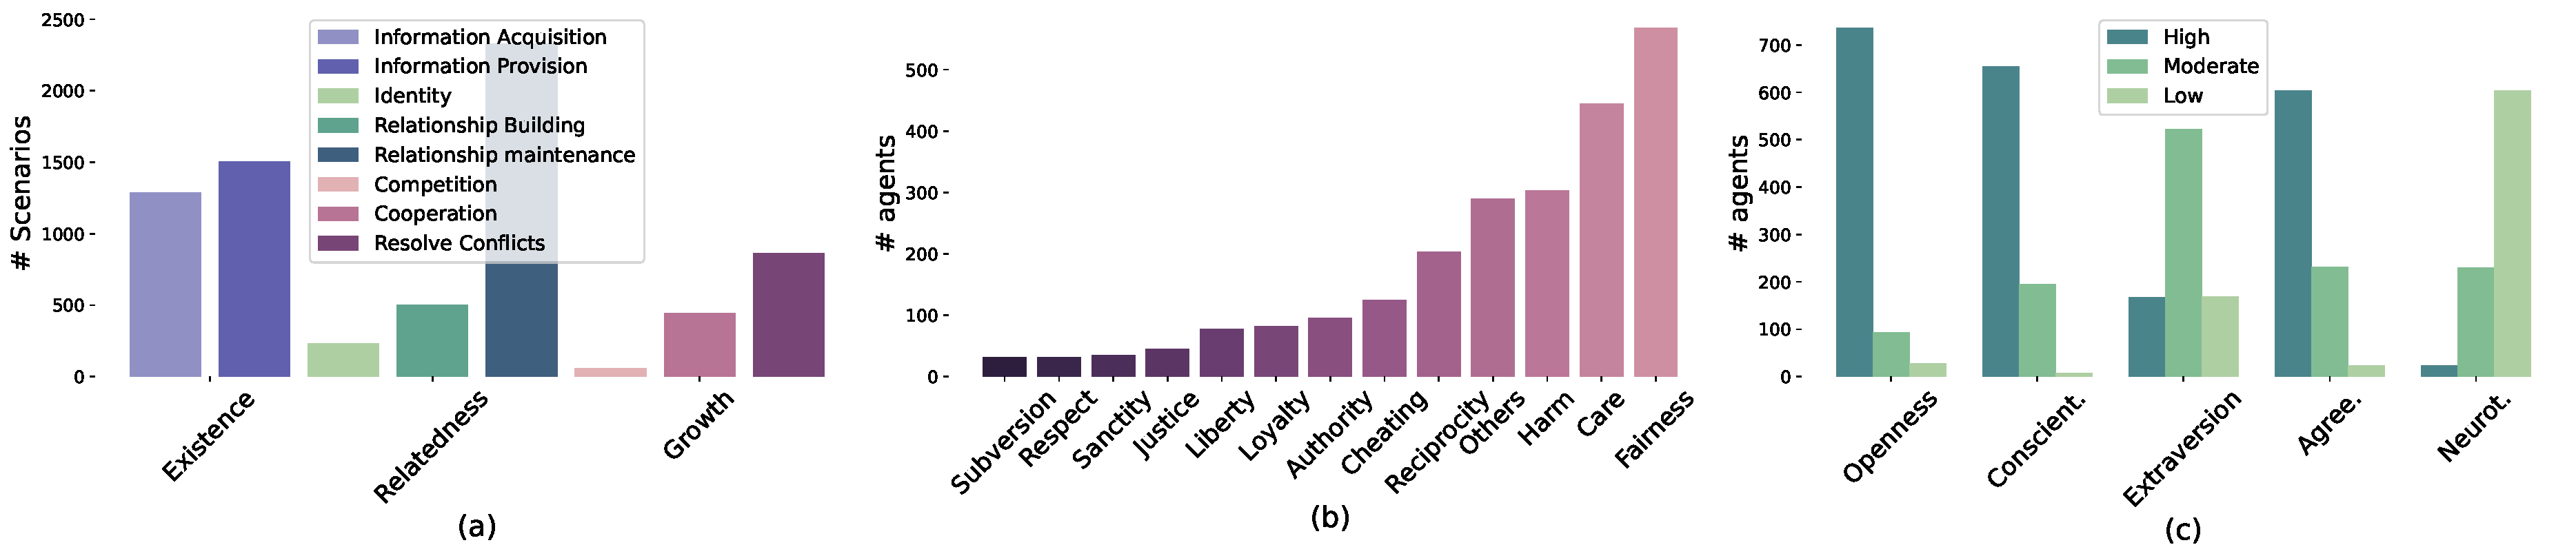
\includegraphics[width=1\textwidth]{latex/figs/merge.pdf}
    \caption{(a) Number of scenarios aligned with the eight categories under ERG theory. Each scenario may encompass multiple goals. (b) Moral values distribution of the agents. An individual may have multiple moral values, with those appearing fewer than 30 times categorized as \textit{Others}. (c) Distribution of the agents' Big Five personality traits. }
    \label{fig:merge}
\end{figure*}